\section{Integration grids generated by Vegas} \label{sec:app-int-grids}

The adaptive algorithm implemented in the \texttt{vegas} package approximates the distributions for each integration variable to improve the evaluations of the integral. From these distributions, different grids for pairs of integration variables can be shown, helping to understand for which points in phase space do higher contributions to the integral occur. The first of these integration grids was shown in \autoref{fig:ex1e_one_grid}, corresponding to the pair of kinematic variables $s$ and $\cos{\theta}$. Since the integrand depends only on these two variables, it is arguably the most insightful one. Here, however, the other two integration grids are shown in \autoref{fig:app-integration-grids} for completeness, as they allow to confirm that \texttt{vegas} did find a uniform distribution along $\phi$. Furthermore, these two integration grids also display more clearly the higher contributions of $s$ for values closer to $M_{\text{Z}}^{2}$, the mass of the Z boson, as well as the asymmetrical contributions for $\cos{\theta}$ towards $+1$ and $-1$, the distribution being slightly more dense towards 1.

\begin{figure}[ht!]
     \centering
     \begin{subfigure}[t]{0.49\textwidth}
         \centering
         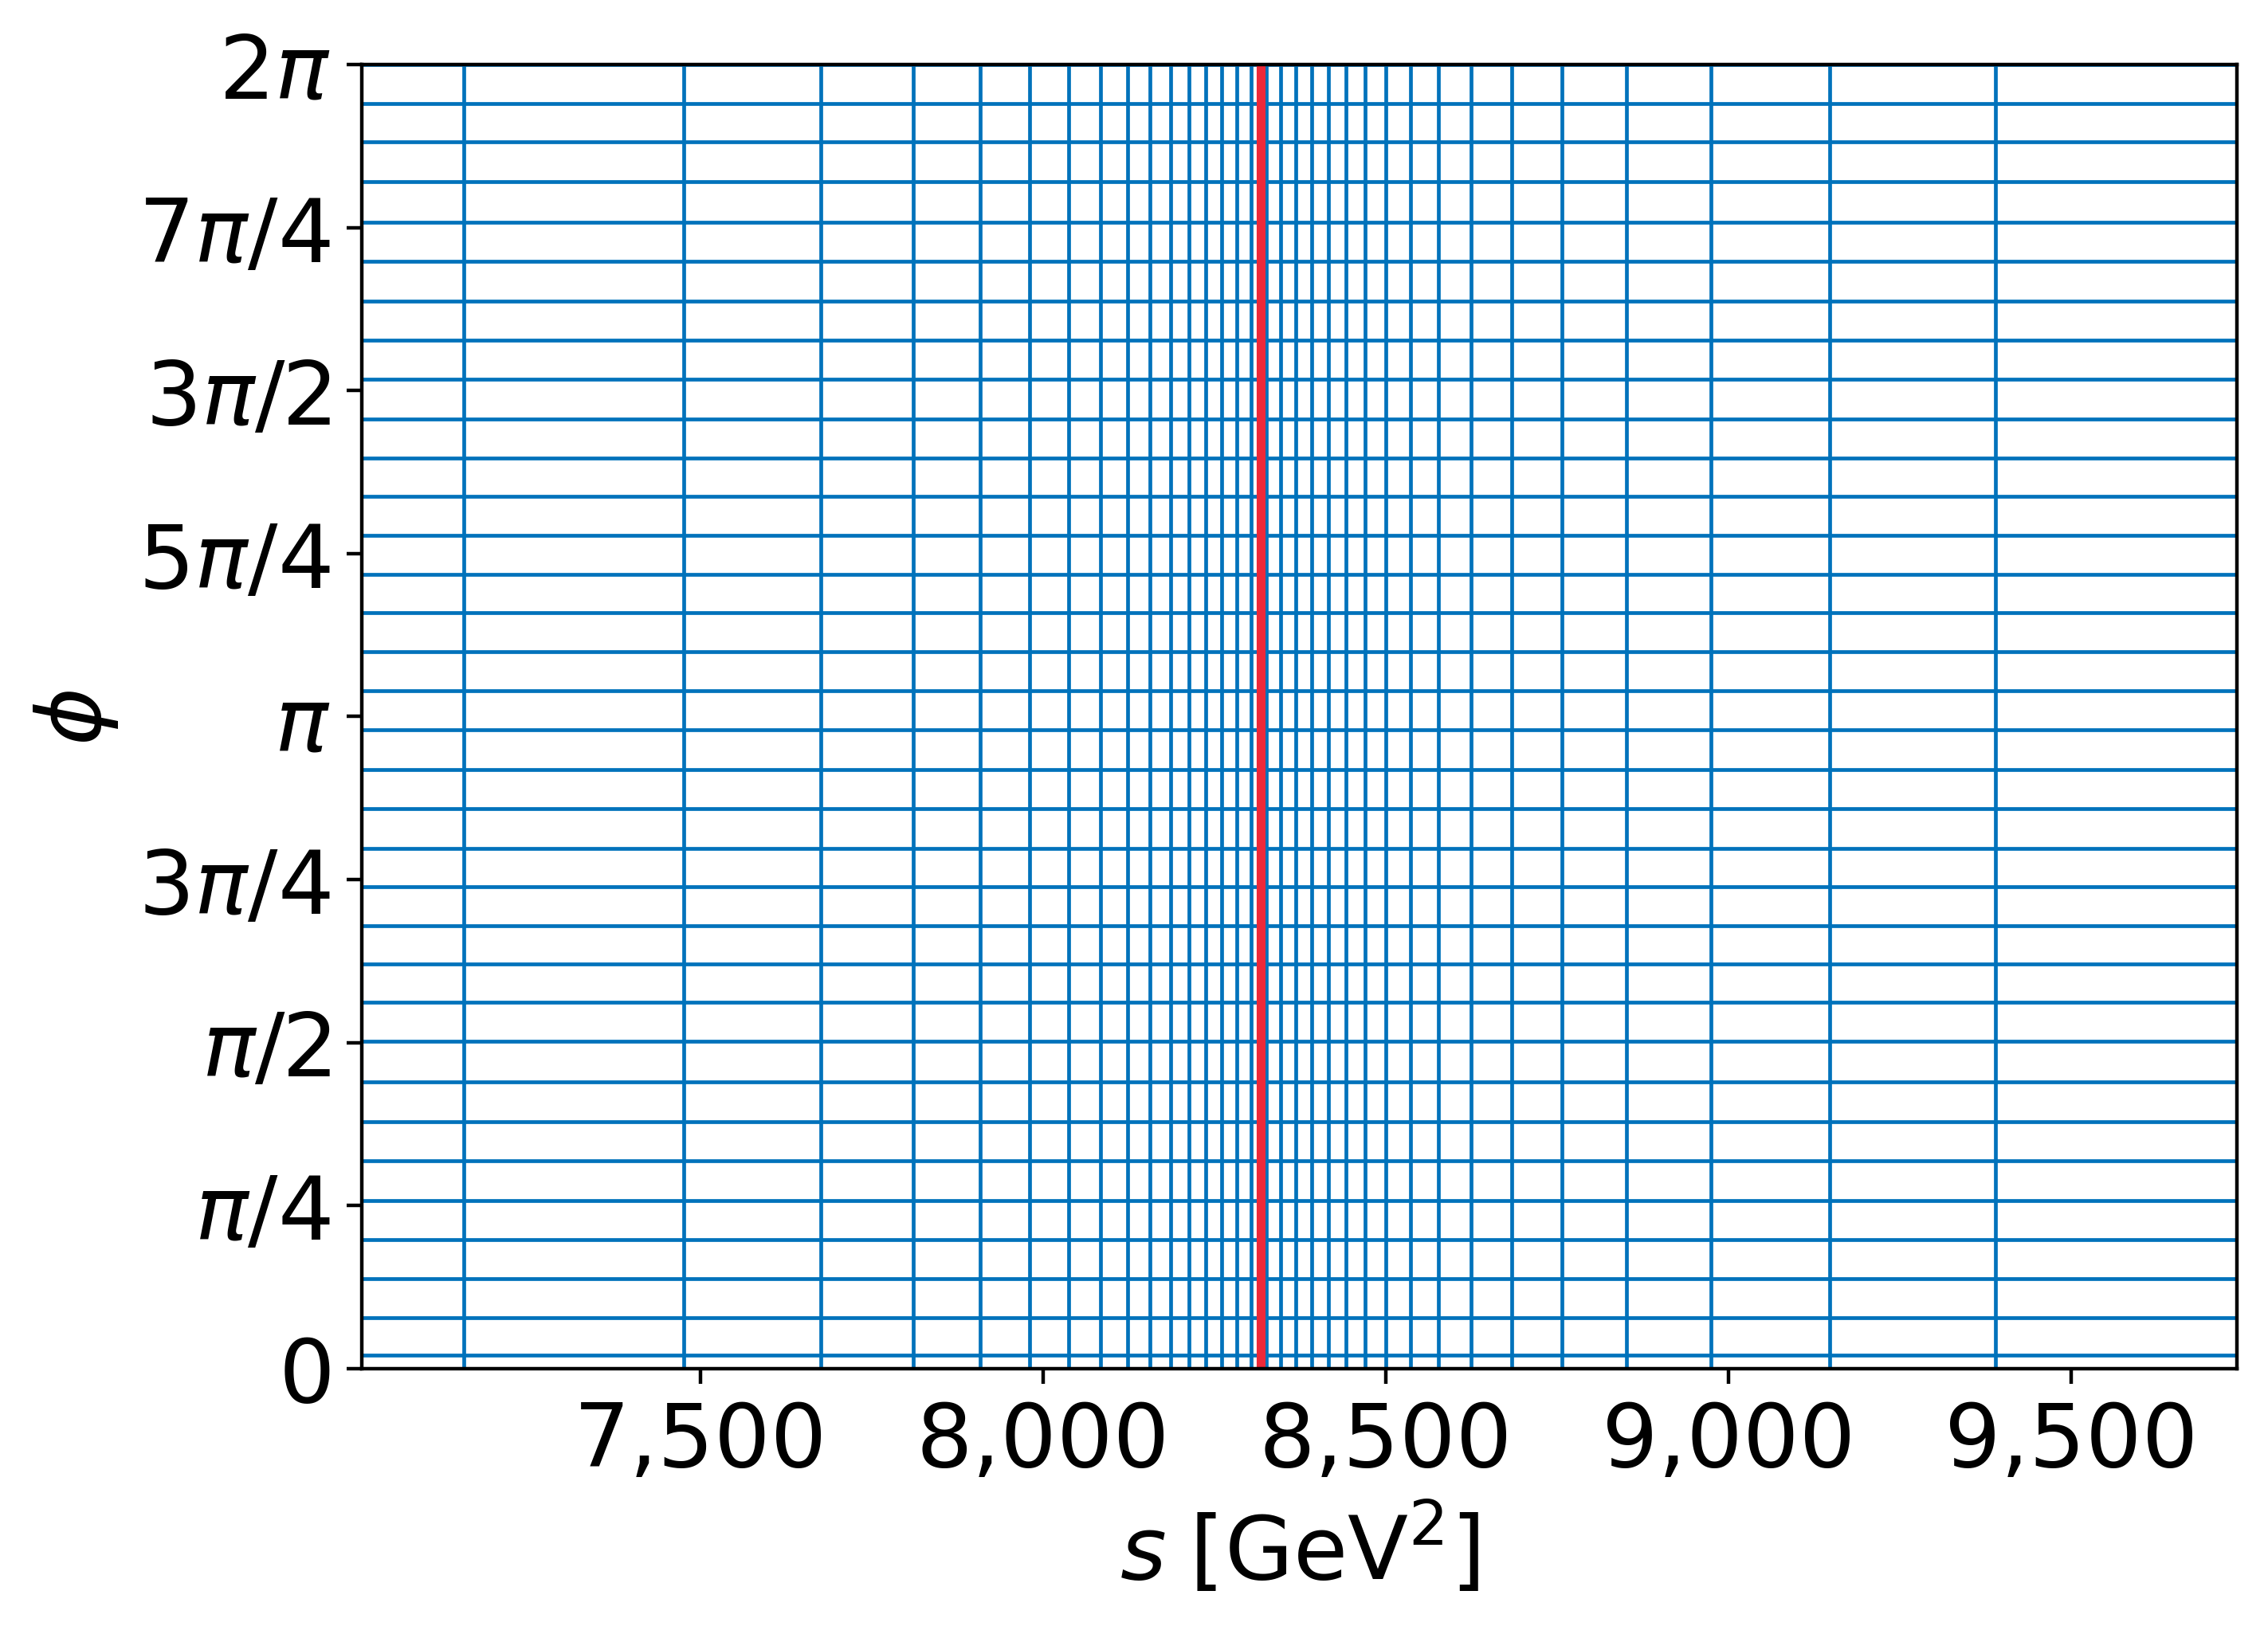
\includegraphics[width=\textwidth]{figures/integration_grid_1.png}
         \caption{}
         \label{fig:app-integration-grid1}
     \end{subfigure}
     \hfill
     \begin{subfigure}[t]{0.49\textwidth}
         \centering
         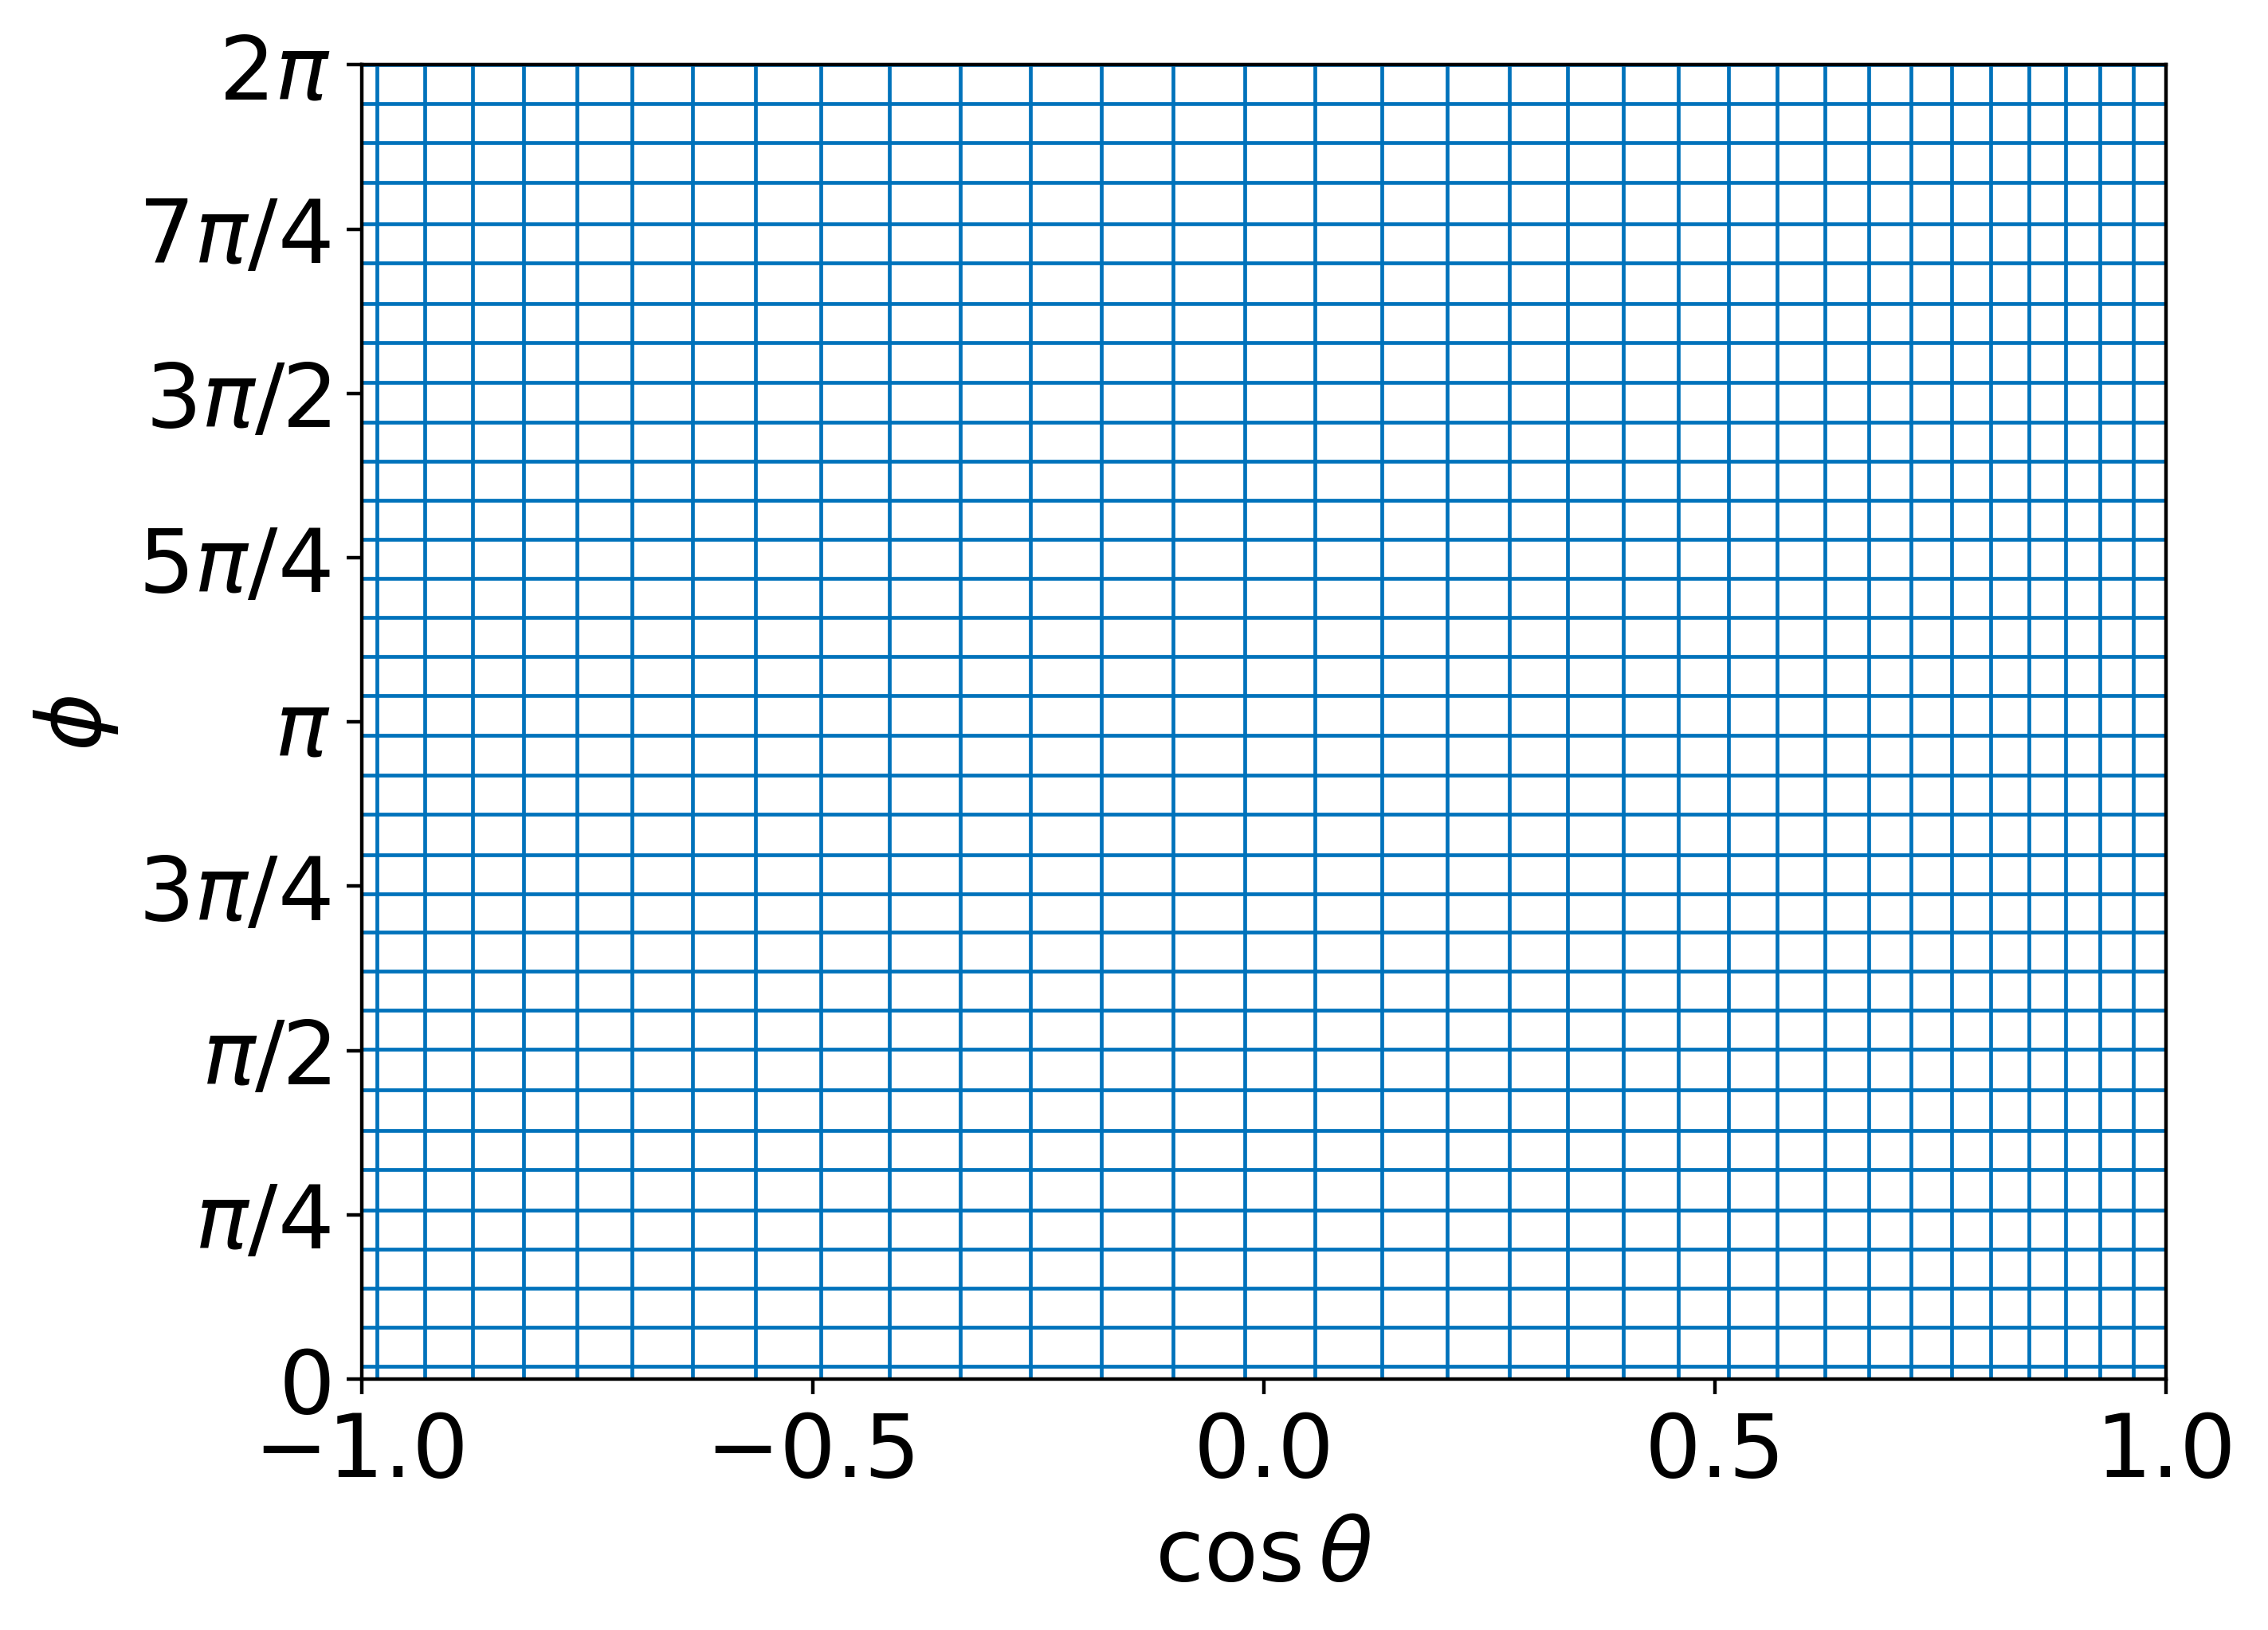
\includegraphics[width=\textwidth]{figures/integration_grid_2.png}
         \caption{}
         \label{fig:app-integration-grid2}
     \end{subfigure}
        \caption{Vegas integration grids for the other two pairs of kinematic variables. The red line corresponds to $s = M_{Z}^{2}$.}
        \label{fig:app-integration-grids}
\end{figure}
